\subsubsection{Information}
\begin{itemize}
	\item \textbf{Course Name:} \href{https://www.coursera.org/learn/start-ux-design-process}{Start the UX Design Process: Empathize, Define, and Ideate}
	\item \textbf{Instructor:} \href{https://www.coursera.org/instructor/google-career-certificates}{Google Career Certificates}
	\item \textbf{Level:} Beginner
	\item \textbf{Enrolled on:} April 4, 2024
	\item \textbf{Finished on:} April 30, 2024
	\item \textbf{Grade Achieved:} 88.75\%
\end{itemize}

\subsubsection{Certificate}
\begin{flushleft}
	\begin{figure}[!ht]
		\centering
		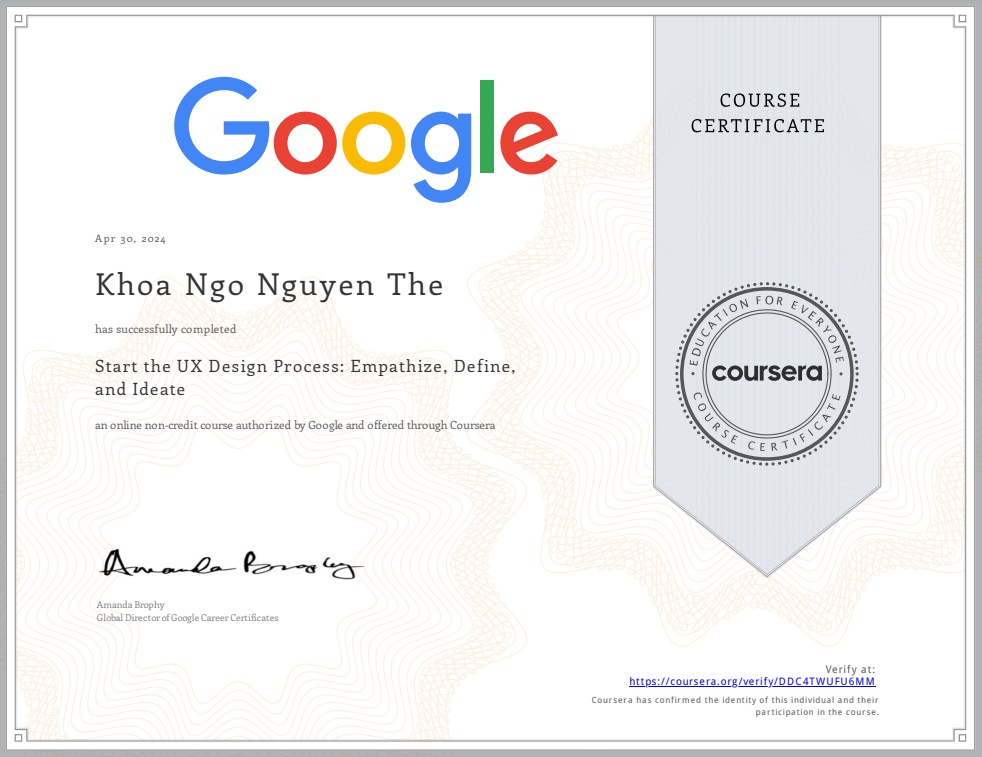
\includegraphics[width=0.85\textwidth]{imgs/Course2.png}
		\caption{Course 2 Certificate}
	\end{figure}

	Visit the online certificate for more info \href{https://www.coursera.org/account/accomplishments/verify/DDC4TWUFU6MM}{here}
\end{flushleft}

\subsubsection{Summary}
\begin{flushleft}
	What I have learned after completing this course:
	\begin{itemize}
		\item Empathize with users to understand their needs and pain points.
		\item Develop problem statements to define user needs.
		\item Generate ideas for possible solutions to user problems.
	\end{itemize}
\end{flushleft}

\subsubsection{Details}
\begin{flushleft}
	\begin{description}
		\item[Module 1:] Empathizing with users and defining pain points
		      \begin{itemize}
			      \item I have thought through the needs of my potential users to build empathy maps and create personas. These hands-on activities helped me understand user perspectives and pain points.
		      \end{itemize}
		\item[Module 2:] Creating user stories and user journey maps
		      \begin{itemize}
			      \item I have continued to empathize with users of the mobile app and crafted user stories and develop user journey maps.
			      \item I have also learnt about the importance of considering accessibility when empathizing with users.
		      \end{itemize}
		\item[Module 3:] Defining user problems
		      \begin{itemize}
			      \item I have moved from the empathize phase into the define phase of the design process.
			      \item To define the problem my designs will solve, I have built a problem statement, a hypothesis statement, and a value proposition.
			      \item In addition, I have explored how psychology and human factors influence design.
		      \end{itemize}
		\item[Module 4:] Ideating design solutions
		      \begin{itemize}
			      \item I have considered everything I've learnt about the users I'm designing for and the problems they're facing in order to brainstorm ideas for design solutions.
		      \end{itemize}
	\end{description}
\end{flushleft}